    \begin{subfigure}[c]{0.45\textwidth}
        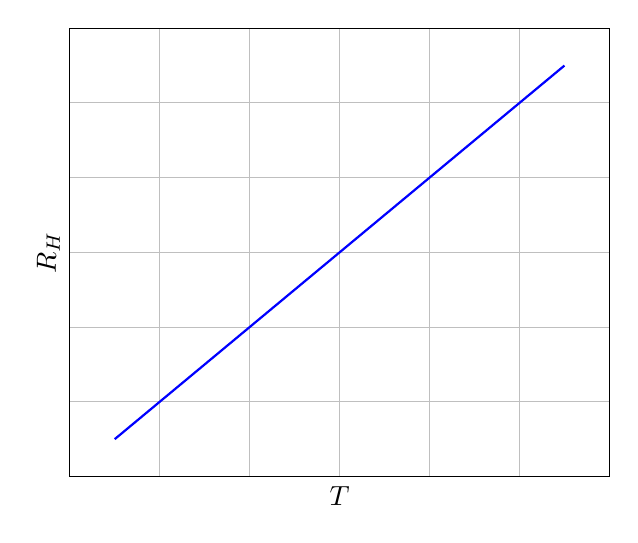
\begin{tikzpicture}
            \begin{axis}[
                ticks=none,
                xlabel={$T$}, ylabel={$R_H$},
                grid=both
            ]
                \addplot[thick, blue] {x};
            \end{axis}
        \end{tikzpicture}
        \caption{Hall-Widerstand}
    \end{subfigure}
    \begin{subfigure}[c]{0.45\textwidth}
        \begin{tikzpicture}
            \begin{axis}[
                ticks=none,
                xlabel={$T$}, ylabel={$R_\square$},
                grid=both
            ]
                \addplot[thick, blue] {1};
            \end{axis}
        \end{tikzpicture}
        \caption{Schichtwiderstand}
    \end{subfigure}
